\documentclass{article}
\usepackage{tikz}
\usetikzlibrary{arrows.meta,arrows}
\usepackage{pgfplots}
\usepackage{xcolor}
\pgfplotsset{compat=1.16}

\begin{document}

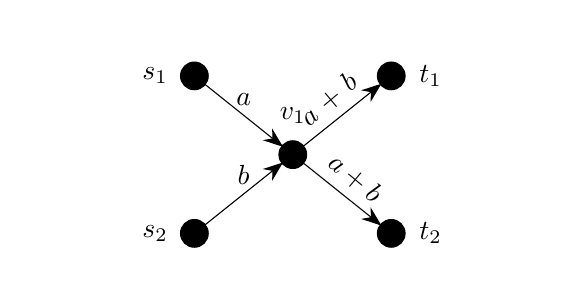
\begin{tikzpicture}
    \draw[fill=black] (0,1) circle (5pt);
    \draw[fill=black] (0,-1) circle (5pt);
    \draw[fill=black] (1.25,0) circle (5pt);
    \draw[fill=black] (2.5,1) circle (5pt);
    \draw[fill=black] (2.5,-1) circle (5pt);
    % nodes
    \node (A) at (0,1) {};
    \node (E) at (0,-1) {};
    \node (D) at (1.25,0) {};
    \node (B) at (2.5,1) {};
    \node (C) at (2.5,-1) {};
    \path [->,-{Stealth[scale=1.5]}]   (A) edge node[midway,above] {$a$} (D); 
    \path [->,-{Stealth[scale=1.5]}]   (E) edge node[midway,above] {$b$} (D); 
    \path [->,-{Stealth[scale=1.5]}]   (D) edge node[midway,above,rotate=40,text width=2cm,align=center] {$a+b$} (B); 
    \path [->,-{Stealth[scale=1.5]}]   (D) edge node[midway,above,rotate=-40] {$a+b$} (C);
    \node (L) at (-0.5,1) [text width=3cm,align=center] {$s_1$};
    \node (L) at (-0.5,-1) [text width=3cm,align=center] {$s_2$};
    \node (L) at (1.25,0.5) [text width=3cm,align=center] {$v_1$};
    \node (L) at (3,1) [text width=3cm,align=center] {$t_1$};
    \node (P) at (3,-1) [text width=3cm,align=center] {$t_2$};
\end{tikzpicture}

\end{document}